\section{Nós e Topologia}

Cada nó sensor integra transdutores, circuitos de condicionamento e aquisição de sinais, unidade de processamento com memória, transceptor sem fio e fonte de energia \cite{AKYILDIZ2002393}.
Nessa estrutura, o microcontrolador controla o ciclo de amostragem, aplica conversões e verificações de plausibilidade, associa marcas temporais às medições e pode executar agregação ou detecção local de eventos antes do envio dos dados \cite{YICK20082292,ANASTASI2009537,5597912}.
Para reduzir a perda de dados durante indisponibilidades breves do enlace, o armazenamento temporário em memória local permite preservar as medições e encaminhá-las após o restabelecimento da comunicação, desde que a capacidade do buffer seja suficiente \cite{5597912,10.1145/1031495.1031521}.

A Figura \ref{fig:no_sensor_ambiental} sintetiza os blocos funcionais descritos.

\begin{figure}[!ht]
    \centering
    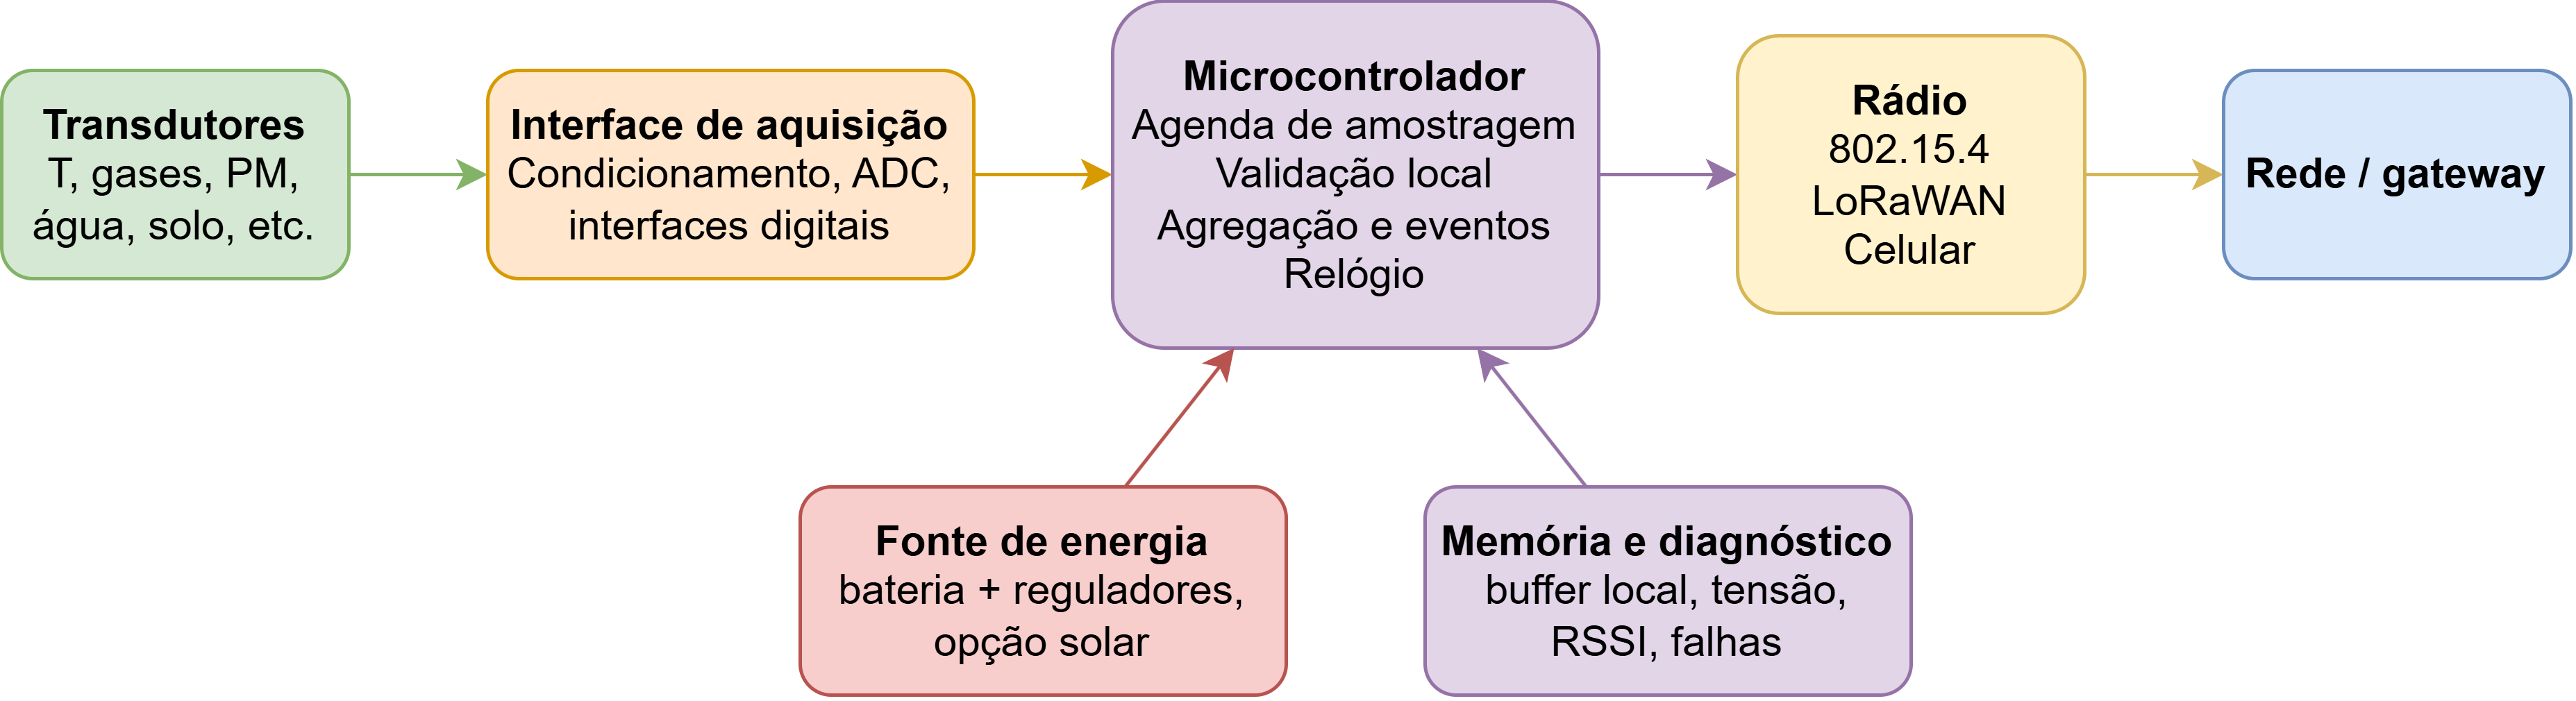
\includegraphics[width=0.98\columnwidth]{figures/blocos_funcionais_sensor_ambiental.drawio.png}
    \caption{Blocos funcionais de um nó sensor ambiental.}
    \label{fig:no_sensor_ambiental}
\end{figure}

A topologia da \ac{RSSF} é definida em função da extensão da área, do relevo, da distribuição dos pontos de medição e das condições de propagação dos enlaces \cite{10.1145/1134680.1134685,5597912}.
Quando todos os nós mantêm enlace direto com o gateway, uma topologia em estrela é adequada. Em topologias multi-hop, o encaminhamento por nós intermediários pode ampliar a cobertura em áreas com obstáculos, porém aumenta o consumo energético e faz a entrega depender da disponibilidade dos nós retransmissores \cite{YICK20082292,ANASTASI2009537,10.1145/1031495.1031521}.
Para aplicações distribuídas por áreas extensas e com baixa taxa de geração de dados, uma LPWAN pode ampliar a área atendida por cada gateway e reduzir a densidade de infraestrutura necessária \cite{7815384}.
Em qualquer dessas configurações, a seleção do protocolo de comunicação depende da análise conjunta do alcance, da taxa de dados, do consumo energético, das condições de propagação impostas pelo relevo e pela vegetação, da infraestrutura disponível e do custo \cite{5597912,7815384,8030482,10.1145/1134680.1134685}.